\chapter{Analysis} \label{ch:analysis}

The following chapter contains the analysis techniques used  as well as developed for analysis from the following experiments:



\section{BRIKEN experiment}

\subsection{YSO }
\subsection{Ion-beta correlations}
\subsection{Calibrations of low- and high-gain branches}


\section{VANDLE experiment}
\subsection{Particle identification}

As mentioned in the experiment section, particle identification is performed by the BigRIPS particle separator using the TOF-B$\rho$-$\Delta$E method. The values of \textit{Z} and \textit{A/Q} are deduced using the measured values of TOF, B$\rho$, and $\Delta$E using the following equations:

The time of flight of a particle for a flight path L:

\begin{equation}\label{eq:1}
TOF = \frac{L}{\beta c}
\end{equation}

Equating Lorentz and centripetal forces experienced by a particle in magnetic field B:

\begin{equation}\label{eq:2}
\frac{A}{Q} = \frac{B \rho}{\beta \gamma} \frac{c}{m_{u}}
\end{equation}


The Bethe-bloch formula describing energy-loss ($\Delta$E) of a particle a material:

\begin{equation}\label{eq:3}
\frac{dE}{dx}=\frac{4\pi e^{4}Z^{2}}{m_{e} \nu^{2}} Nz \Bigg[ ln \frac{2m_{e} \nu^{2}}{I} -ln(1-\beta^2) -\beta^{2}\Bigg],
\end{equation}


Here $\beta=\nu/c$, $\gamma = 1/ \sqrt{1-\beta^2}$) is the velocity of the particle, $m_{u}$ = 931.4 MeV is the atomic mass unit, $m_{e}$ is the electron mass, and e is the electron charge. z, N and I represent the atomic number, atomic density and mean excitation of the material, respectively. $\textit{Z, A}$ and \textit{Q} denote the proton number, atomic mass, and charge states of a fragment, respectively.


move the Bigrips picture here:

Now from the diagram of the BigRIPS separator we can see that the flight path L is from F3 to F7, and is measured by thin plastic scintillators located at F3 and F7. The foci at F3 and F7 are fully achromatic, while the ones at F1 and F5 are momentum dispersive. $\Delta$E is measured by using the multi-sampling ionization chamber (MUSIC) located at F7. The $B \rho$ measurement is done using the trajectory reconstruction from F3-F5 and from F5-F7. The trajectory of the particles is tracked with the help of a position-sensitive parallel plate avalanche counters (PPAC) located at F3, F5, and F7. 

The PPAC detectors and the energy degrader at F5 lead to energy loss. Hence, $B \rho$ measurements are done for F3-F5 path and F5-F7 path. The leads to a change in equations \ref{eq:1} and \ref{eq:2} as follows:

\begin{equation} \label{eq:4}
TOF = \frac{L_{35}}{\beta c_{35}} + \frac{L_{57}}{\beta c_{57}}
\end{equation}


\begin{equation}\label{eq:5}
\left (\frac{A}{Q} \right)_{35} = \frac{B \rho_{35}}{\beta_{35} \gamma_{35}} \frac{c}{m_{u}}
\end{equation}


\begin{equation}\label{eq:6}
\left (\frac{A}{Q} \right)_{57} = \frac{B \rho_{57}}{\beta_{57} \gamma_{57}} \frac{c}{m_{u}}
\end{equation}


If the charge state of the ion does not change on its course from F3 to F7 at F5. We will have the following relation by equating \ref{eq:5} and \ref{eq:6}: 


\begin{equation}\label{eq:7}
\frac{B \rho_{35}}{B \rho_{57}} = \frac{\beta_{35} \gamma_{35}}{\beta_{57} \gamma_{57}}
\end{equation}


The velocities of the fragments before and after F5 can be deduced using equations \ref{eq:4} and \ref{eq:7} from the measured TOF and $B\rho_{35,57}$ values. The absolute value of $\textit{Z}$ can be then deduced using by modifying equation \ref{eq:3} as follows:

\begin{equation}\label{eq:8}
Z = a \beta \sqrt{\frac{\Delta E}{ln \left (\frac{2m_{e} c^2 \beta^2}{I} \right ) -ln(1-\beta^2) -\beta^{2}}} + b
\end{equation}

where the inputs to the equation are $\Delta E$ and $\beta_{57}$, a and b are the parameters that need to be determined during the experiment from calibrations.

In the follwoing sections we show the cuts and gates implemented in the data for building cleaner events tagged with calibrated \textit{Z} and \textit{A/Q}.


\subsubsection{F3 and F7}

Plastic scintillator detectors located at F3 and F7 for measuring TOF are readout using the photomultplier tubes (PMT), which are coupled to the left and right ends of the detector. The position of an incident particle can be found using the charge-integrated signals $q_{1}$ and $q_{2}$ from left and right end of the detector using the following expression:

\begin{equation}\label{eq:9}
x = -\dfrac{\lambda}{2} ln \left ( \dfrac{q_{1}}{q{2}} \right ).
\end{equation}


Here, $\lambda$ denotes the attenuation length of scintillation light in the detector. We can also get the position from the timing of the left and right PMT siganls as 

\begin{equation}\label{eq:10}
x = -\dfrac{V}{2}(t_{2}-t_{1})
\end{equation}

By equating Eqs \ref{eq:9} and \ref{eq:10} we got the basis for rejecting signals in the data lying far-off from the constraint defined by the following equation:

\begin{equation}\label{eq:11}
-\dfrac{\lambda}{2} ln \left ( \dfrac{q_{1}}{q{2}} \right ) = \dfrac{V}{2}(t_{2}-t_{1})
\end{equation}

where V denotes the propagation speed of light in the scintillation counter. Figure \ref{fig:F3_plastic_cut} and \ref{fig:F7_plastic_cut} shoes the correlation derived from time-difference and the ratio of the left and right PMT signal amplitudes from the data.

\begin{figure}[h]
	\centering
	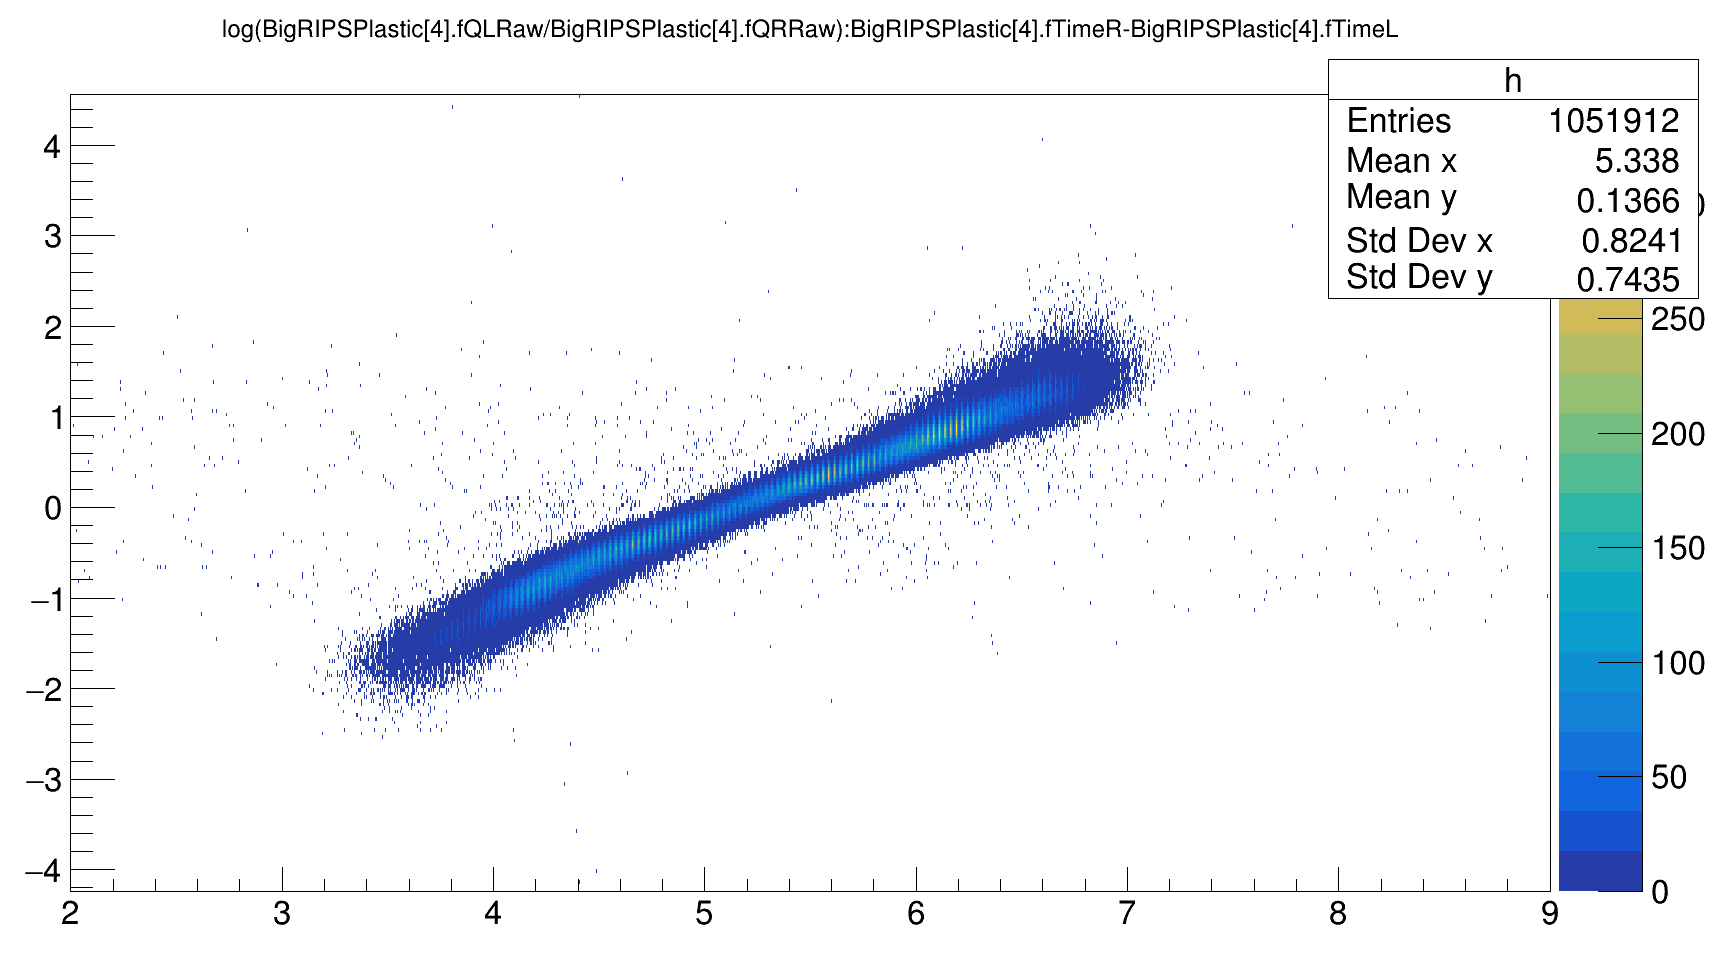
\includegraphics[width=6cm,height=4cm]{figures/F3_plastic_cut.png}
	\caption[Implementation of cuts at F3 plastic to reject background events.]{Implementation of cuts at F3 and F7 plastic to reject background events.}
	\label{fig:F3_plastic_cut}
\end{figure}

\begin{figure}[h]
	\centering
	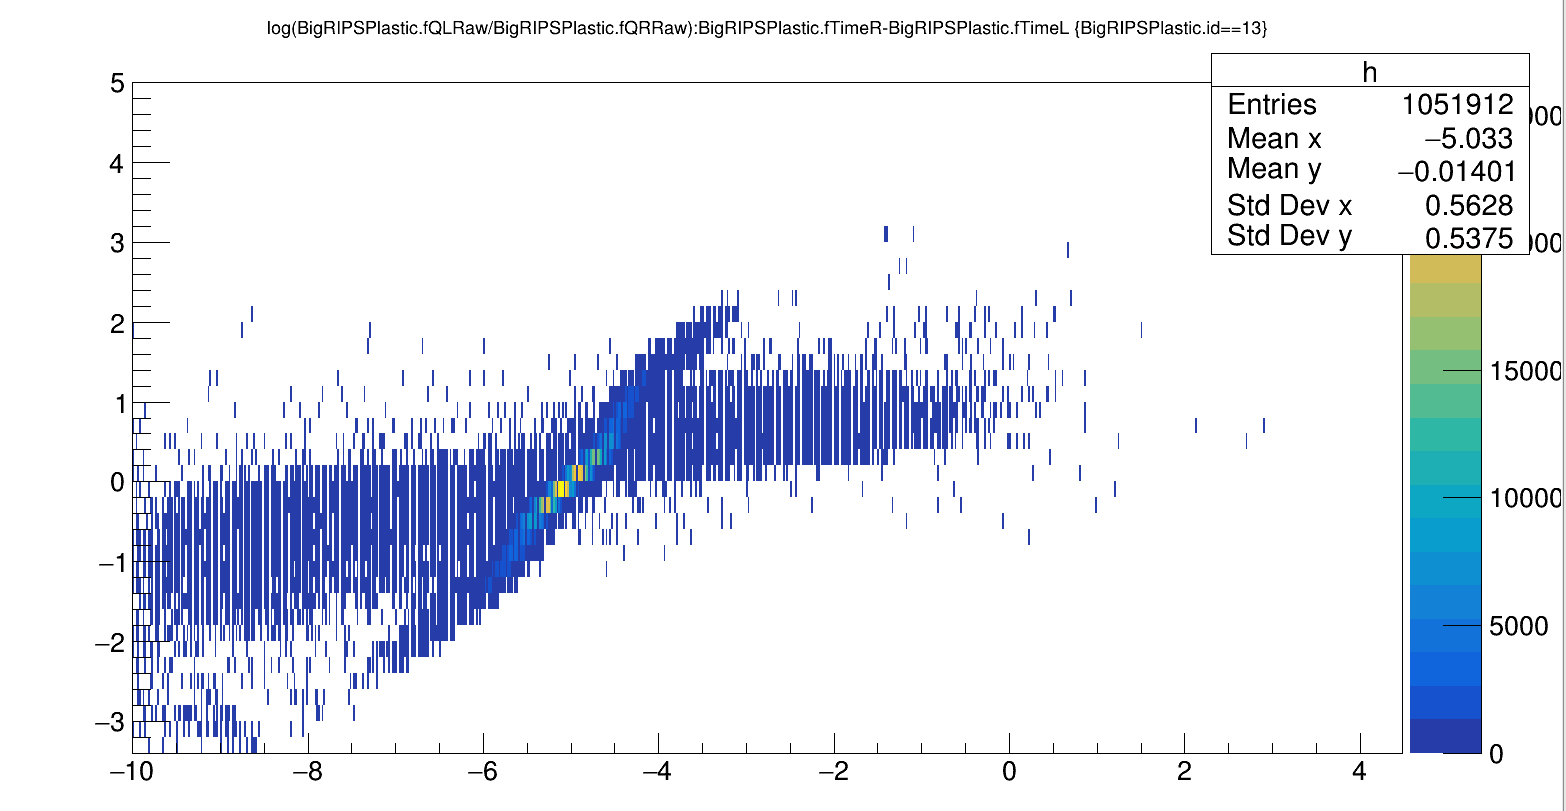
\includegraphics[width=6cm,height=4cm]{figures/F7_plastic_cut.png}
	\caption[Implementation of cuts at F7 plastic to reject background events.]{Implementation of cuts at F3 and F7 plastic to reject background events.}
	\label{fig:F7_plastic_cut}
\end{figure}

\subsubsection{PPAC}

The position-sensitive Parallel Plate Avalance Counter (PPAC) are used for tracking the fragments in the beamline at RIBF. The detector consist of several plates with 4 readouts ($T_{X_{(1, 2)}}$ and $T_{Y_{(1, 2)}}$) for position tracking. The detectors adopt a delay-line readout method [N FUKUDA]. The position of an incident particle is determined from the time difference between two timing signals $T_{1}$ and $T_{2}$ obtained from the ends of the delay line in the PPAC detector. The sum of the timing defined as 


\begin{equation}
T_{sum} = T_{1} + T_{2},
\end{equation}

remains constant independent of the position of the incident particle, and acts as an important tool to remove inconsistent events and effects of $\delta$-rays from the data.

\begin{figure}[h]
	\centering
	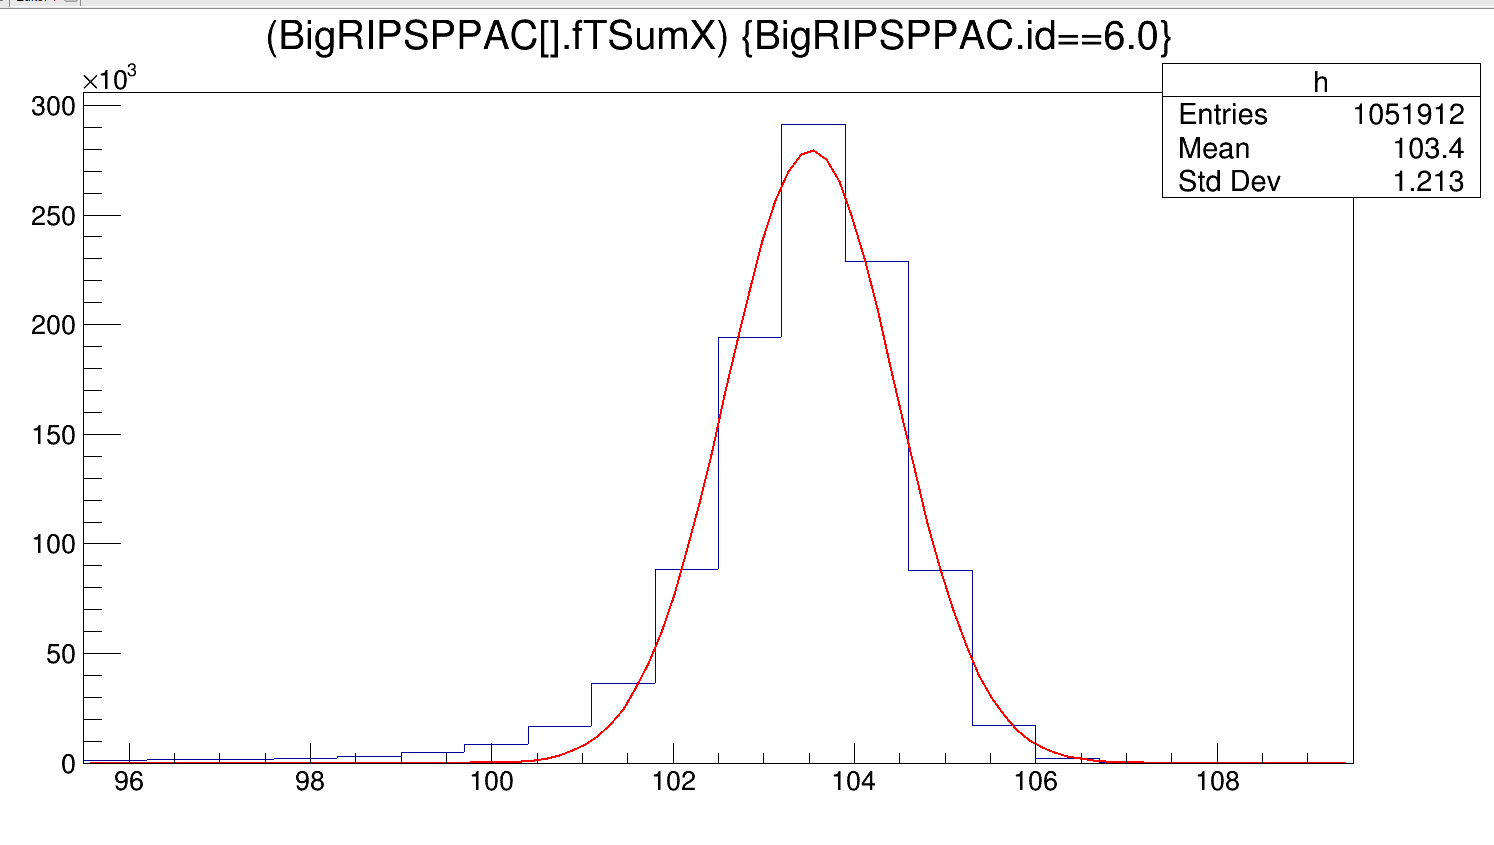
\includegraphics[width=8cm,height=6cm]{figures/PPAC_cut.png}
	\caption[]{$T_{sum}$ for the sum of one of the plates of PPAC at F3. Only events lying within the FWHM range of the main peak are accepted. }
	\label{fig:PPAC_cut}
\end{figure}

As an example, Figure \ref{fig:PPAC_cut} shows the $T_{sum}$ distribution for \textit{X} position signals of one of the plates of PPAC located at F3. Similar cuts were used for all the PPAC detector plates in the BigRIPS separator.

 
 
\subsubsection{MUSIC ($\Delta$E) detector}

The MUSIC detector used for the $\Delta$E measurement in the BigRIPS separator consists of twelve anodes and thirteen cathodes aligned alternately. The neighboring anodes are electrically connected in pairs. The six anode signals are read independently and averaged for the $\Delta$E measurement. The fragments on their way through the MUSIC detector can cause nuclear reactions with the electrodes and the counter gas. The correlation between alternative anodes helps to remove inconsistent events from the beam. 

\begin{figure}[h]
	\centering
	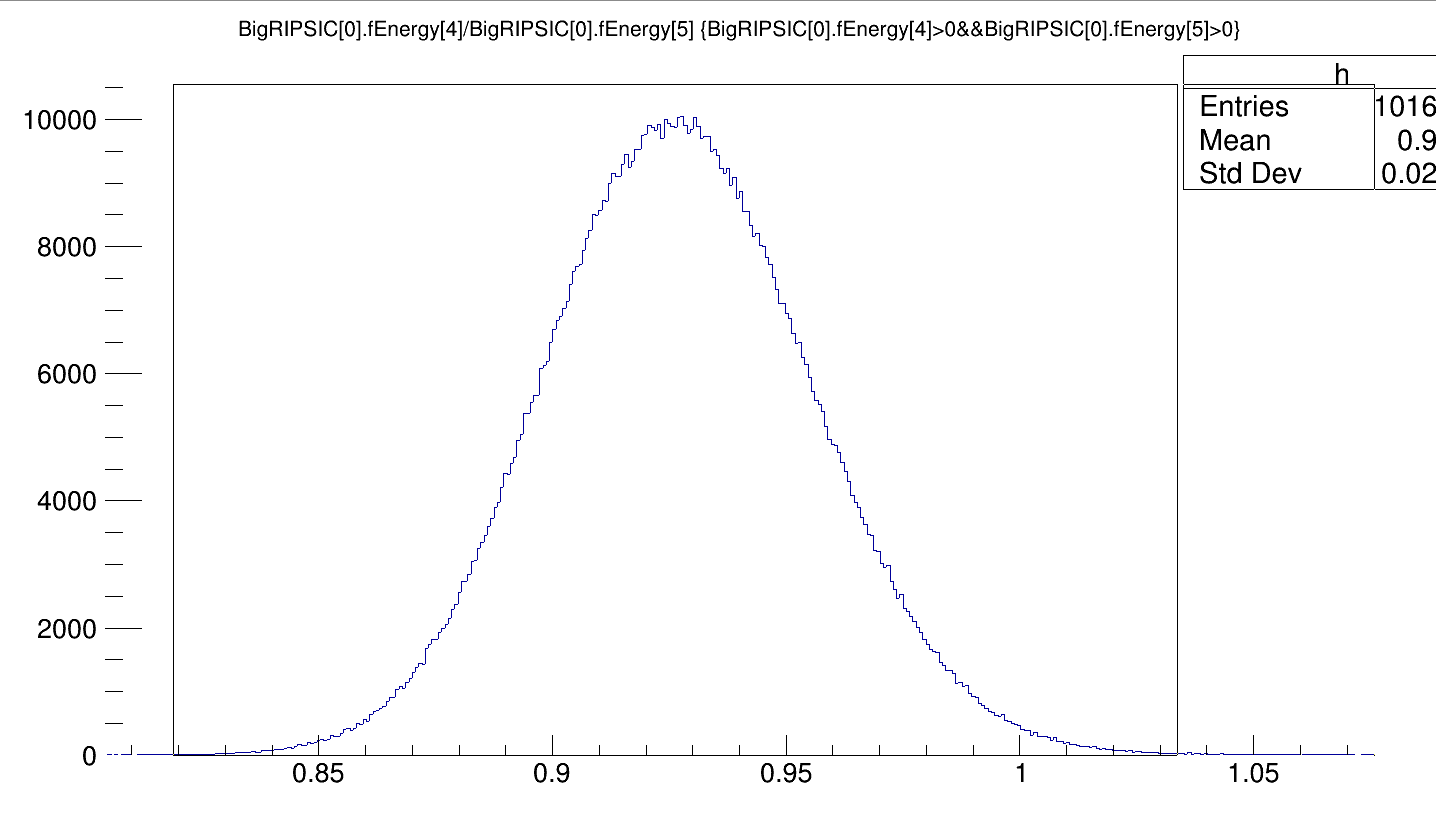
\includegraphics[width=10cm,height=6cm]{figures/MUSIC_detector.png}
	\caption[]{Ratio of 5th and 4th anode signal for the MUSIC detector.}
	\label{fig:MUSIC_cut}
\end{figure}

As an example, Figure \ref{fig:MUSIC_cut} shows the ratio of signals from two consecutive anodes. The signals were accepted within the FHWM of the peak of the distribution. Similar gates were implemented for all the consecutive anode signals.

\begin{figure}[h]
	\centering
	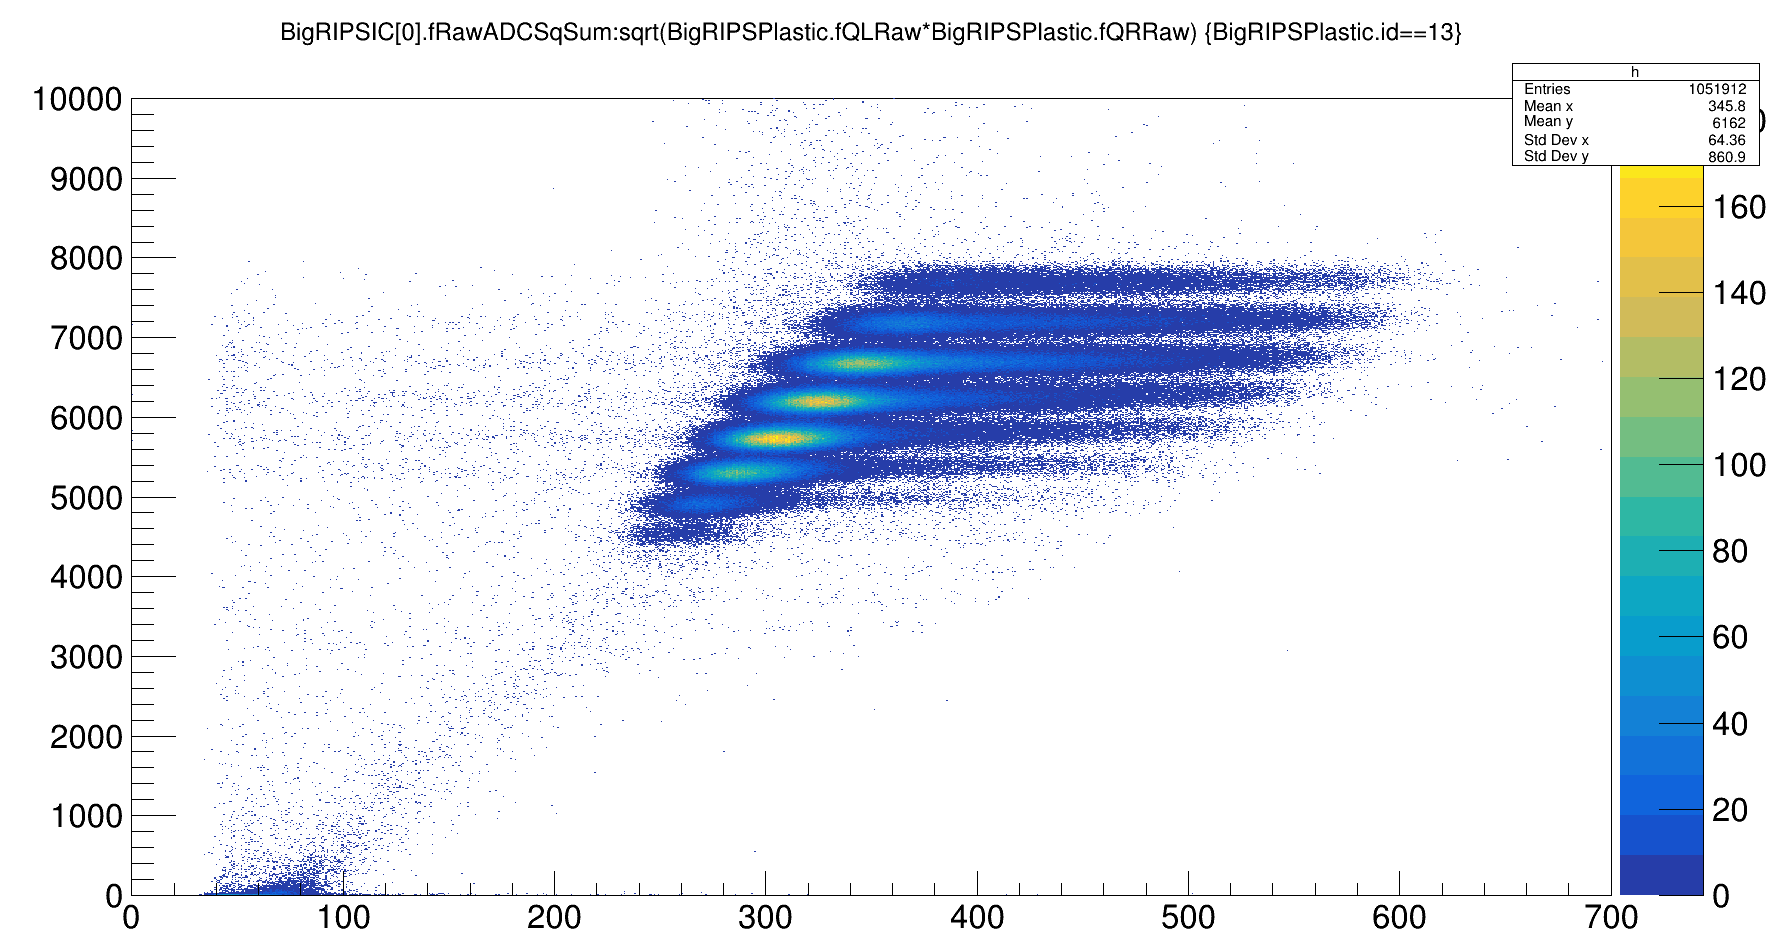
\includegraphics[width=10cm,height=6cm]{figures/F7_MUSIC.png}
	\caption[]{}
	\label{fig:F7_MUSIC}
\end{figure}

Further, fragments upon leaving F7 plastic can have a change in the charge state due to reactions in the F7 plastic. These events were rejected using correlation between the signal from the MUSIC detector and the signals from the left and right of the F7 plastic as shown in Figure \ref{fig:F7_MUSIC}.




The source of noise in data was identified to be in the F7 plastic as shown in Figure \ref{fig:F7_Plastic}. Upon the implementation of all these a liner function for calibration of \textit{Z} used. 


\begin{figure}[h]
	\centering
	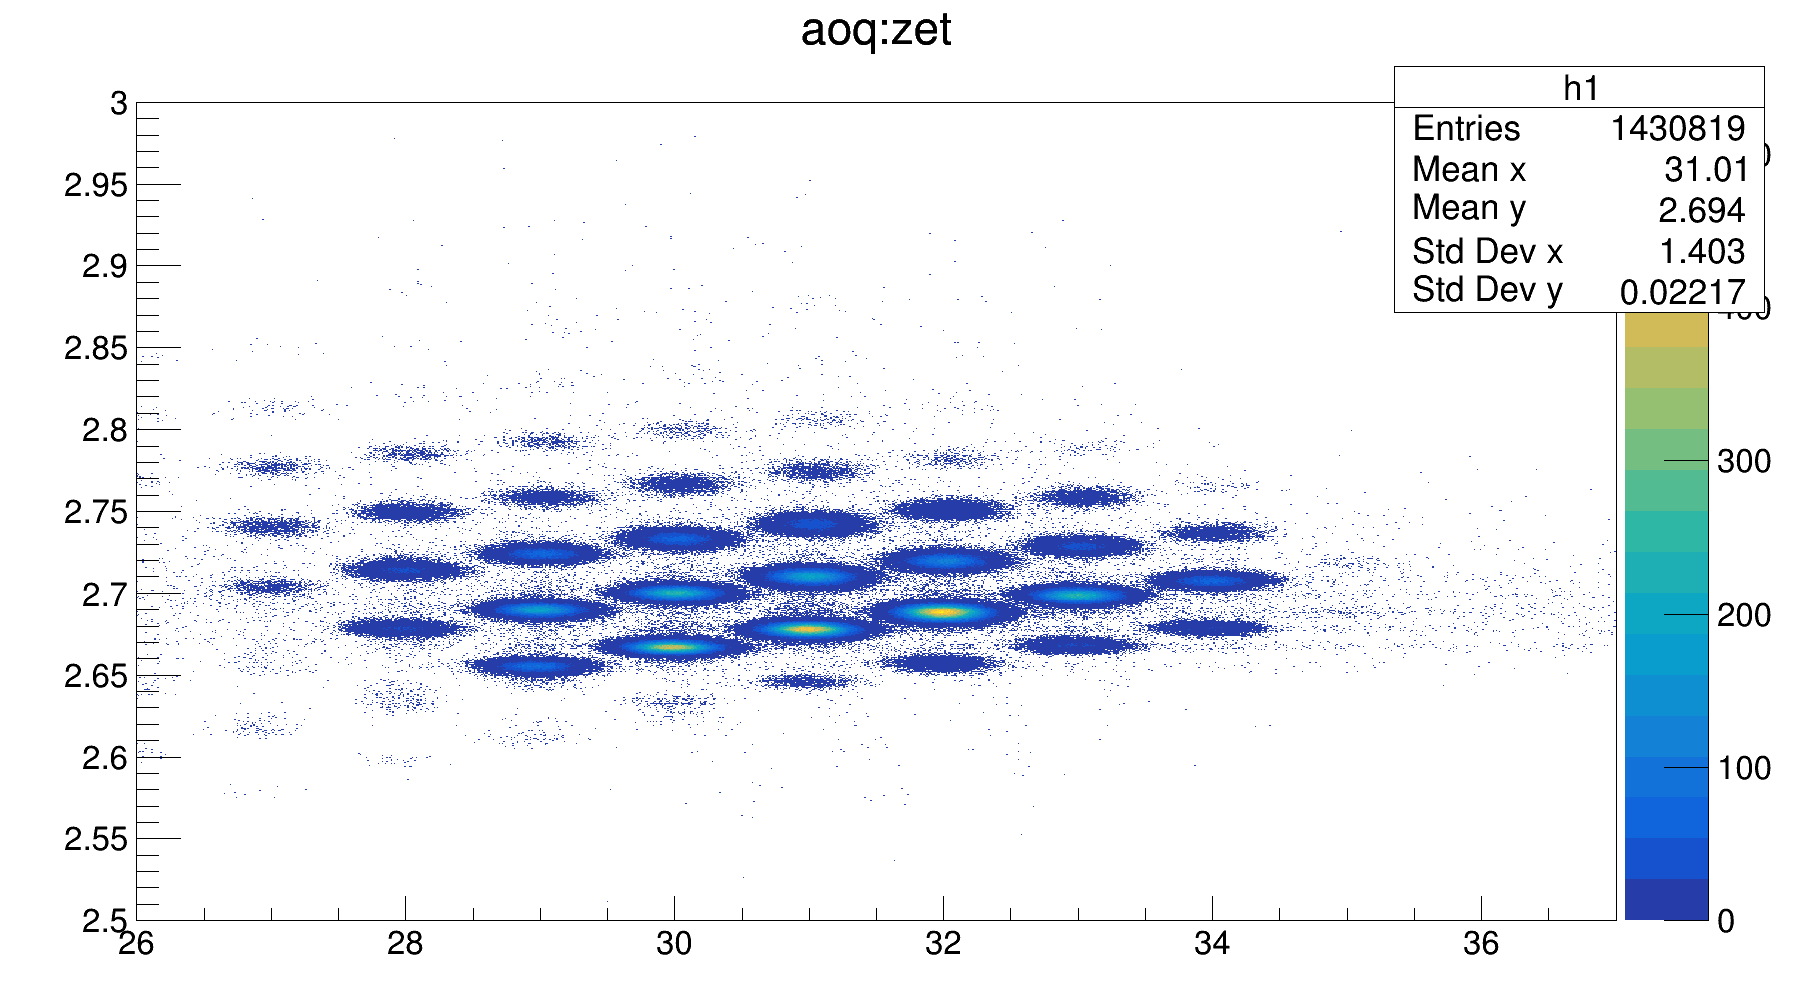
\includegraphics[width=10cm,height=6cm]{figures/PID_uncleaned.png}
	\caption[]{}
	\label{fig:PID_uncleaned_F7}
\end{figure}


\begin{figure}[h]
	\centering
	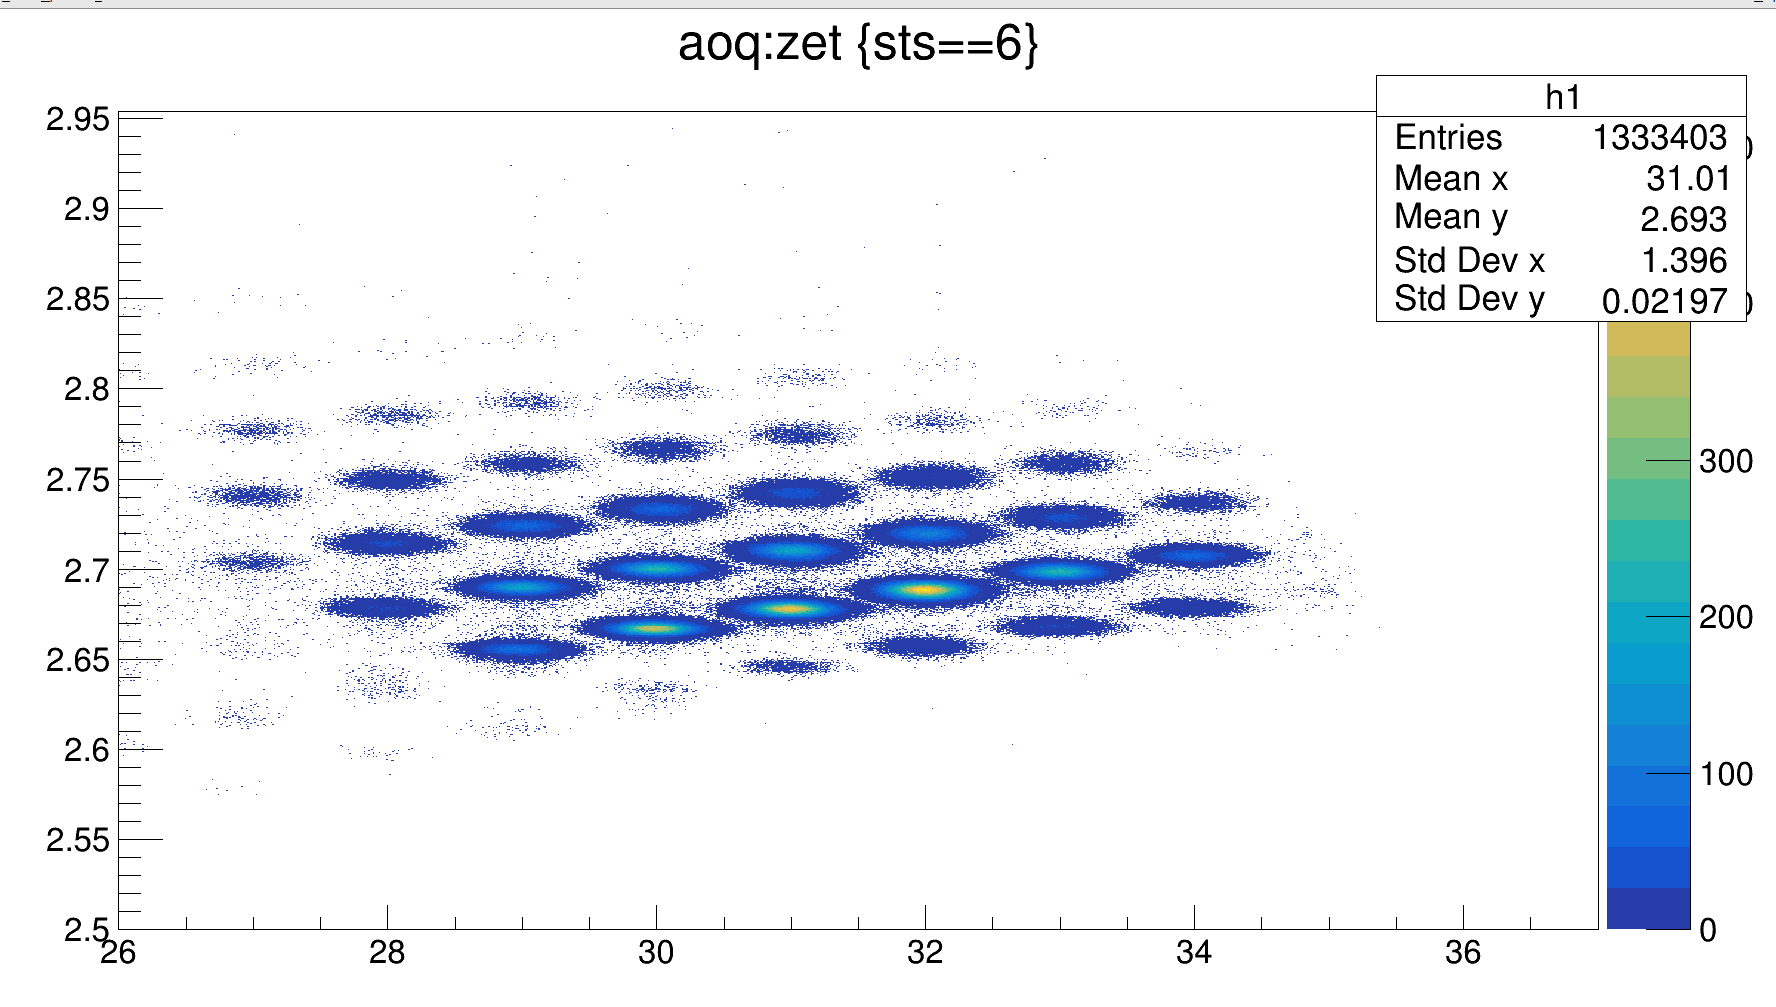
\includegraphics[width=10cm,height=6cm]{figures/PID_cleaned.png}
	\caption[]{}
	\label{fig:PID_cleaned_F7}
\end{figure}

\newpage

\section{Clovers}

The main analysis for clovers constituted of calibration and efficiency calculations. A clover detector contains 4 HPGe crystals sensitive to $\gamma$-rays. The crystals need to be calibrated individually followed by proper gain-matching to get a good resolution. For efficiency and calibration data were collected using standard sources in the experiment configuration. Calibrated sources, such as $\textsuperscript{133}$Ba, $\textsuperscript{60}$Co, $\textsuperscript{137}$Cs, and $\textsuperscript{152}$Eu were used for efficiency measurements. Some of the crystals of the clovers suffered from gain shift during the experiment. Thus, calibration parameters from the source run could not be implemented for the experiment runs. However, a number of known background lines were identified in the in-beam runs and they were used for calibration. The lines are listed below along with their sources.

/*VERIFY from the cheat sheet in the office*/
\begin{center}
	\begin{tabular}{ |c|c|c| } 
		\hline
		$\gamma$-ray (keV) & Source \\
		\hline
		351.9 & $\textsuperscript{214}Pb(Ra)$ \\ 
		511 & Pair production \\ 
		788.7 & $\textsuperscript{138}La$ \\ 
		1435.7 & $\textsuperscript{138}La$ \\ 
		1460.8 & $\textsuperscript{40}K$ \\ 
		1764.5 & $\textsuperscript{214}Bi(Ra)$ \\ 
		2614.7 & $\textsuperscript{208}Tl(Th)$ \\ 
		\hline
	\end{tabular}
\end{center}

A polynomial of first order as shown in equation \ref{eq:clover_calibration} was used to calibrate clover spectrum to keV.
\begin{equation} \label{eq:clover_calibration}
E_{\gamma} = a*E_{ch} + b
\end{equation}
Here, a and b represent the calibration parameters.



The YSO detector is sensitive to $\gamma$-rays and acts a $\gamma$-ray absorber. Hence, this can lead to a lowering of $\gamma$-ray efficiency, more adversely for low-energy $\gamma$-rays. To properly account for the absorption effects from the YSO and for the sake of accuracy, efficiency for clovers was measured by placing a standard source for the mentioned list at different position on the face of the YSO detector. Figure \ref{fig:YSO_source_holder} shows the layout the source holder and this source holder was affixed onto the face of the YSO detector to quantify change in the efficiency with a change in the position of a gamma source in the YSO detector.

\begin{figure}[h]
	\centering
	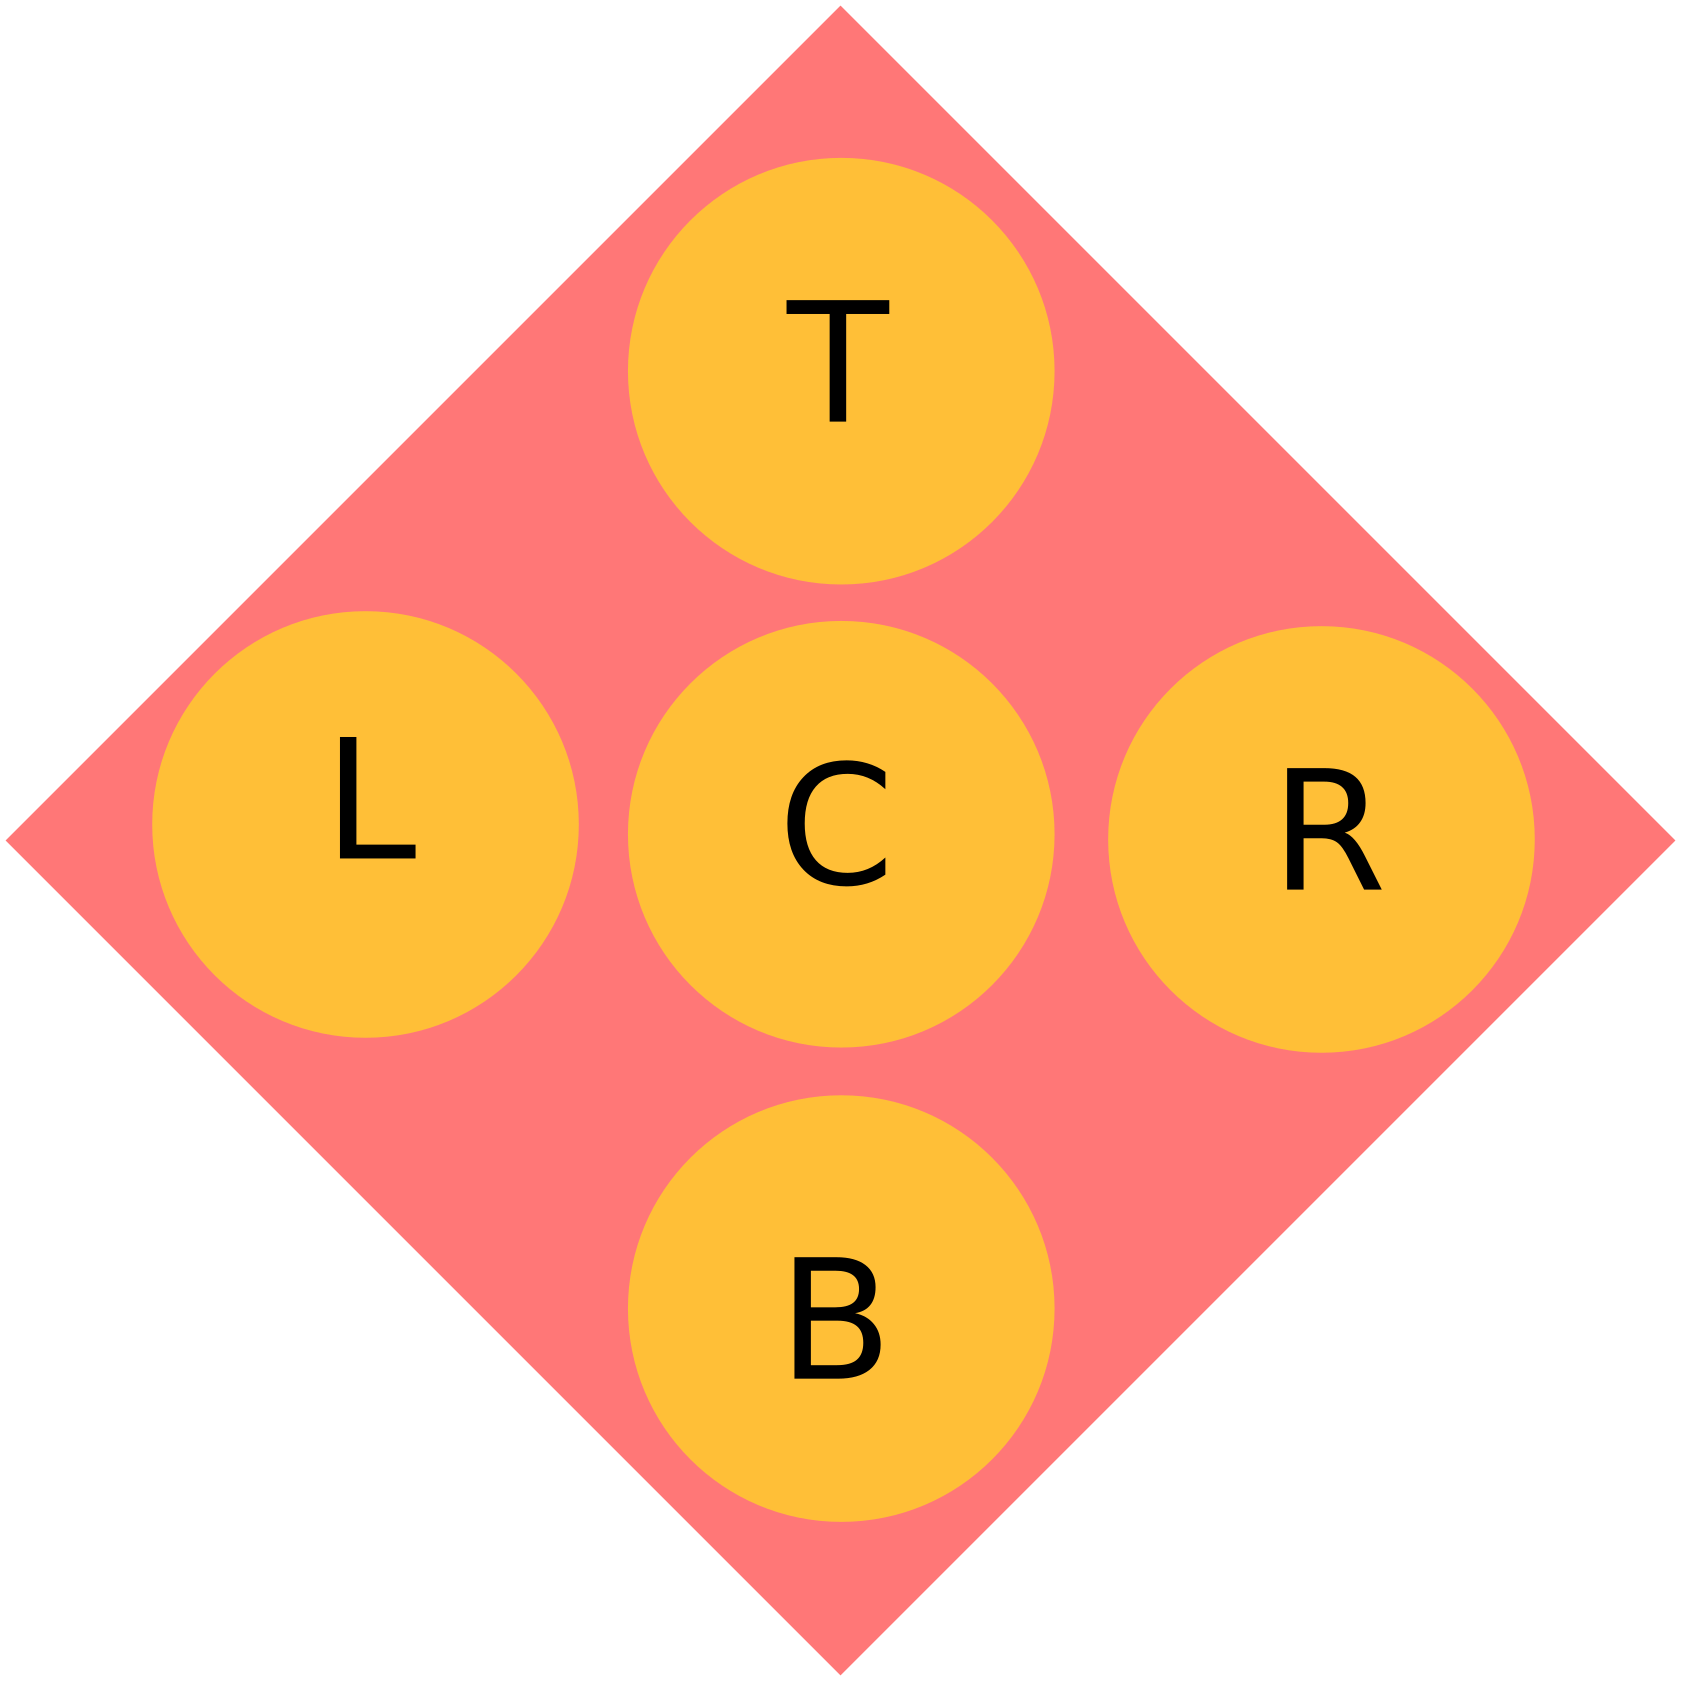
\includegraphics[scale=0.5]{figures/Yso_source_holder.png}
	\caption[]{Design of a 3D-printed source holder matching the dimensions of the YSO. Yellow circles show cavities for placing a source. The source positions are labeled as top (T), bottom (B), left (L), right(R), and center (C). }
	\label{fig:YSO_source_holder}
\end{figure}


Further, from the efficiency measurements it was seen that the data from $\textsuperscript{152}Eu$ was subjected to significant dead time due to high source activity. The dead time then leads to a underestimation of the efficiency. The dead time was calculated using count rate for 1435.7-keV line from $\textsuperscript{138}La$. The ratio of the count rate from the background and the source data gives the required scaling needed for the main peaks in the source run.Figure \ref{fig:1435_7_background} shows the dead time for all the source runs. $\textsuperscript{152}Eu$ suffers from most of the dead time. The same count rate was calculated for in-beam runs,and it showed no dead time.

\begin{figure}[h]
	\centering
	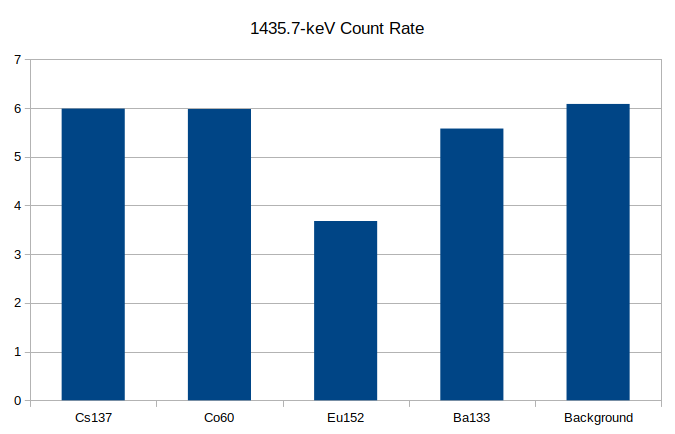
\includegraphics[scale=0.5]{figures/background_count_rate.png}
	\caption[]{Dead time across all the source runs.}
	\label{fig:1435_7_background}
\end{figure}


The data collected for the efficiency measurements was later used to benchmark a GEANT4 simulation package. The 
benchmark here is to get a reliable efficiency measurements from the GEANT4 when a source is place at any position on the face of the YSO detector. The criterion adopted for the benchmark  was to have efficiency from the simulations within the error bars at each for measurements at each of the positions or there is a discrepancy no more than $\sim$ 5-8 $\%$ between the data and the simulations. Also, a number a simulations were run to find a position for the center of the YSO crystal relative to the clovers in the simulation software setup to meet the criterion.

\begin{figure}[h]
	\centering
	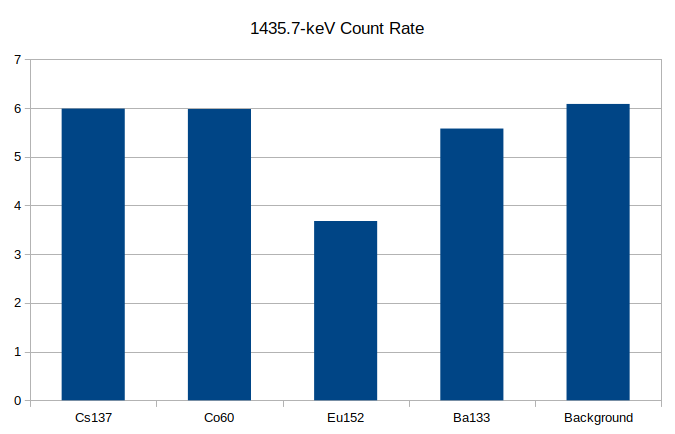
\includegraphics[scale=0.5]{figures/background_count_rate.png}
	\caption[]{Dead time across all the source runs.}
	\label{fig:1435_7_background}
\end{figure}









	
	


\*Mention explicitly all the algorithms used for the analysis*\
\subsection{Data Streams Merging}
\subsection{YSO Analysis Development}
\subsection {Dynamic Range Tests}
\subsubsection{Reconstruction of ion and beta distributions}
\subsection{Comparison of Gates showing background and dynode-single energy curve}
\subsection{Properties of the PSPMT, Vertilon Board and the light guide used}
\subsection{Put electronics diagrams of both the PSPMT and the board, elaborate the working in a reductive manner; split the paragraphs before}
\subsection{Development of algorithm for ion-beta correlations}
\subsubsection{Beta Background Quantify}
\subsection{Bateman equation fitting for Cu80}
\subsection{Explanation for counting betas for the beta delayed neutron emitters using the bateman equations}
\subsection{Bateman equation fitting for Ga83}
explain the shape of the decay curve 
\subsection{VANDLE Analysis}
\subsubsection{Efficiency Measurements}
\subsection{Americium Measurement}
\subsection{Time Calibration}
\subsection{Walk Characteristics}
\subsubsection {Walk Correction for YSO and VANDLE}
Explain the methodology as you filled in the sheet.
\subsection{Flight Path Reconstruction using implant position coordinates}
\subsection{Cu81 neutron spectrum}

Analysis will include preparation of ion-beta timing gate

\subsection{Cu80 neutron spectrum}
\subsection{Cu79 neutron spectrum}




Plot graphs with the ratios of the timing corrected and uncorrected to gauge the position of YSO.

Talk about the technique to find the offset.

\subsection{Neutron Background Subtraction Techniques}
\subsection{Neutron Calibration}
\subsection{YSO light quenching Estimates}

Explain the process for the YSO light quenching
Calibration
low-gain branch calibration in MeVee
quenching factors for various isotopes 
Lise++ plots showing kinetic energy distribution

\section{Gamma-ray Analysis}
\subsubsection{Addback}
\subsubsection{Efficiency characterization using GEANT4}
Main points would be describe the characterization of the efficiency/bench-marking.
Technique developed to get efficiency estimates using implant position and using gamma efficiency on an event-by-event basis. 
\subsubsection{HaGRID}

\section{GEANT4 simulations}

\subsection{VANDLE efficiency from simulations}

\subsection{Explain the estimates of efficiency}
\subsection{Explain the bench-marking process for the simulation}
\subsubsection{Gain Adjustment of the VANDLE PMT}
\subsubsection{Response Function development}

discuss the anatomy and the shape of the function. Discuss the shape of the function and the reflection from the top of the function.
\subsection{Estimates for the threshold using data for single bar}
\subsection{}

\subsection{Need for simulations}
Explain with respect to understanding the scattering and affects from various components from the decay station. Need to extract the response

Explain the affect of the YSO in the setup

Import the pictures for scattering positions for the ions in the setup.

Give details of the response function and its anatomy used in the analysis.

Show the fitting of the function for a particular case

Write the equations for various parameters

plot the qdc ratio to extract position using scatter positions


\section{Analysis of \textsuperscript{81,80,79}Cu}
\subsection{Ion-beta correlation}
\subsection{Beta-gated Gamma-ray spectrum}
\subsection{Neutron-gamma Coincidence}
Go in step wise order for the whole data analysis.
Give a general overview of the decay for the whole isotope.

(graphics use DNP 2020 Cu81 as an example.)

Explain the need and how it helps assigning strength for all excited energy levels.
\subsection{De-convolution of neutron spectrum}
Show the histogram here and the calculated peaks.

\subsection{BGT formation}
calculations
\section{discussions}

Write about the results of the analysis
\section{}
